\documentclass[conference]{IEEEtran}
\IEEEoverridecommandlockouts
% The preceding line is only needed to identify funding in the first footnote. If that is unneeded, please comment it out.
\usepackage{cite}
\usepackage{amsmath,amssymb,amsfonts}
\usepackage{algorithmic}
\usepackage{graphicx}
\usepackage{textcomp}
\usepackage{xcolor}
\def\BibTeX{{\rm B\kern-.05em{\sc i\kern-.025em b}\kern-.08em
    T\kern-.1667em\lower.7ex\hbox{E}\kern-.125emX}}
\begin{document}

\title{Learning-Augmented Control for Quadrotor MPC in MuJoCo: When a Feedforward Residual Architecture Helps, Hurts, or Does Nothing}

\author{\IEEEauthorblockN{1\textsuperscript{st} Given Name Surname}
\IEEEauthorblockA{\textit{dept. name of organization (of Aff.)} \\
\textit{name of organization (of Aff.)}\\
City, Country \\
email address or ORCID}
\and
\IEEEauthorblockN{2\textsuperscript{nd} Given Name Surname}
\IEEEauthorblockA{\textit{dept. name of organization (of Aff.)} \\
\textit{name of organization (of Aff.)}\\
City, Country \\
email address or ORCID}
\and
\IEEEauthorblockN{3\textsuperscript{rd} Given Name Surname}
\IEEEauthorblockA{\textit{dept. name of organization (of Aff.)} \\
\textit{name of organization (of Aff.)}\\
City, Country \\
email address or ORCID}
\and
\IEEEauthorblockN{4\textsuperscript{th} Given Name Surname}
\IEEEauthorblockA{\textit{dept. name of organization (of Aff.)} \\
\textit{name of organization (of Aff.)}\\
City, Country \\
email address or ORCID}
\and
\IEEEauthorblockN{5\textsuperscript{th} Given Name Surname}
\IEEEauthorblockA{\textit{dept. name of organization (of Aff.)} \\
\textit{name of organization (of Aff.)}\\
City, Country \\
email address or ORCID}
\and
\IEEEauthorblockN{6\textsuperscript{th} Given Name Surname}
\IEEEauthorblockA{\textit{dept. name of organization (of Aff.)} \\
\textit{name of organization (of Aff.)}\\
City, Country \\
email address or ORCID}
}

\maketitle

\begin{abstract}
Nonlinear Model Predictive Control (MPC) achieves accurate trajectory tracking for quadrotors when the prediction model matches the plant, but degrades when the plant drifts from the nominal model due to mass changes, aerodynamic drag, motor lag, or sensing delay. This paper studies a feedforward residual control architecture that augments a nominal MPC with a small learned correction acting only on the vertical thrust channel. The full pipeline is implemented in MuJoCo using the Skydio X2 quadrotor model. A two hidden layer multilayer perceptron with 5{,}641 parameters is trained on 88{,}500 transitions collected across 21 perturbation configurations, achieving validation R-squared above 0.97 on the three velocity components. The architecture is evaluated against four perturbation types using identical sweeps. On mass perturbations the residual recovers 80 to 92 percent of the tracking error across a 0.7 to 1.4 mass factor range. On linear drag the recovery is approximately zero because drag manifests on horizontal axes that the single-channel correction cannot address. On motor lag the residual is neutral below a cliff at 43 ms and actively increases tracking error by 15 to 29 percent within a narrow transition zone before the cliff. The findings characterize a clean partition between matched, mismatched, and out-of-regime perturbations and quantify a destabilization mode of feedforward residual learning near closed-loop stability boundaries.
\end{abstract}


\begin{IEEEkeywords}
component, formatting, style, styling, insert
\end{IEEEkeywords}

\section{Introduction}

\subsection{Motivation and Background}
Quadrotor unmanned aerial vehicles operate in regimes where unmodeled dynamics dominate tracking performance. Aerodynamic drag becomes significant at speeds above a few meters per second, payload changes shift the effective mass, electronic speed controllers introduce first-order lag on motor commands, and onboard estimation pipelines introduce sensing delay. Nonlinear Model Predictive Control (MPC) is the modern standard for trajectory tracking on this platform because it can plan over a finite horizon while respecting actuator constraints \cite{faessler2018differential, torrente2021data, salzmann2023real}. However, an MPC controller is only as accurate as its internal prediction model. When the plant diverges from the prediction model, the resulting closed loop exhibits degradations that range from graceful and bounded to catastrophic and abrupt, depending on which axis of the dynamics is perturbed and how strongly.
A natural response is to augment the controller with a learned residual that captures the gap between the nominal prediction and the observed evolution \cite{saviolo2023learning, torrente2021data, hewing2020learning}. Two architectures have emerged for integrating such a residual into MPC. The first embeds the learned function inside the optimization as part of the dynamics constraint, which allows the optimizer to anticipate the residual over its prediction horizon. The second applies the residual as a feedforward correction outside the optimizer, which sacrifices anticipation but sidesteps the numerical difficulties of placing a neural network inside an interior-point solver. The first formulation is theoretically attractive but practically fragile, particularly on resource-constrained platforms and within general-purpose interior-point solvers such as IPOPT \cite{wachter2006implementation, andersson2019casadi}. The second is robust and easy to deploy but its competence across perturbation types has not been systematically characterized.

\subsection{Research Statement}
This work asks a single empirical question. Given a learned residual model that accurately predicts one-step dynamics mismatch in simulation, how much of the closed-loop tracking degradation caused by mass, drag, motor lag, and time delay perturbations can a feedforward residual architecture recover, and what specifically limits this recovery? The question is not whether the residual model is accurate in isolation, because that is straightforward to verify on held-out data. The question is whether the residual, when actually applied as a control correction inside a closed loop, helps the controller track better, fails to help, or makes things worse, and whether the answer depends on the perturbation type.

\subsection{Research Objectives}
The investigation pursues four objectives.
\begin{itemize}
\item Characterize the degradation behavior of a nominal quadrotor MPC under four perturbation types (mass, drag, motor lag, time delay) using a controlled simulation harness in MuJoCo \cite{todorov2012mujoco}.
\item Train a small learned residual model on rollout data spanning the perturbation regimes characterized above, and verify its predictive accuracy on held-out validation data.
\item Implement two integration strategies for the residual: an in-constraint formulation that embeds the residual inside the MPC dynamics constraint, and a feedforward formulation that applies the residual as an external thrust correction.
\item Evaluate the feedforward architecture by running the same perturbation sweeps with and without the residual correction, reporting the recovered fraction of the tracking error gap for each perturbation type.
\end{itemize}

\subsection{Contributions}
This paper makes three contributions.
\begin{itemize}
\item A reproducible perturbation characterization of a baseline quadrotor MPC across four distinct mismatch types in a high-fidelity simulator, with all degradation curves and cliff transitions resolved.
\item A diagnosed failure mode of in-constraint residual MPC under warm-started IPOPT, in which a feasible standalone solve does not generalize to a stable closed loop despite multiple rounds of solver tuning, motivating the pivot to a feedforward architecture.
\item A perturbation-wise evaluation of feedforward residual control, reporting 80 to 92 percent gap closure on mass, approximately zero gap closure on drag, and a quantified destabilization effect of 15 to 29 percent above the nominal degraded error in the narrow transition zone of motor lag immediately before the cliff. The destabilization finding identifies a regime in which feedforward residual learning is not merely ineffective but actively harmful.
\end{itemize}
The remainder of the paper is organized as follows. Section II reviews related work on MPC for quadrotors and learning-augmented control. Section III presents the quadrotor model and the MuJoCo simulation environment. Section IV describes the nominal MPC baseline. Section V characterizes the four perturbation types. Section VI describes the learned residual model and its training. Section VII presents the feedforward residual control architecture and discusses the failed in-constraint attempt. Section VIII reports the evaluation. Section IX discusses findings and limitations. Section X concludes.

\section{Related Work}

\subsection{Model Predictive Control for Quadrotors}
Model Predictive Control for quadrotor trajectory tracking has been studied extensively over the past decade. Early formulations focused on linearizing the quadrotor dynamics around hover and applying linear MPC, which is computationally cheap but accurate only in slow flight regimes \cite{kamel2017linear}. Nonlinear MPC formulations followed, treating the full Euler dynamics or quaternion attitude representation symbolically and solving the resulting nonlinear program with interior-point or sequential quadratic programming methods. The introduction of CasADi \cite{andersson2019casadi} and its tight integration with IPOPT \cite{wachter2006implementation} made it practical to compile and solve nonlinear MPC problems for quadrotors in real time on conventional embedded hardware. Faessler et al.\ provided a thorough treatment of differential flatness in the presence of rotor drag and demonstrated that incorporating drag into the prediction model significantly improves agile flight \cite{faessler2018differential}. The dominant modern formulation for trajectory tracking is a cascaded structure in which an outer nonlinear MPC operates on a reduced position-and-attitude state and outputs total thrust together with desired body rates, while a high-bandwidth inner loop tracks the rate references \cite{faessler2018differential, sun2022comparative}. The work presented here adopts this standard cascaded formulation without modification, allowing the comparison between the nominal controller and the residual-augmented variant to isolate the contribution of the learned residual alone.

\subsection{Learned Dynamics for Quadrotor Control}
Two broad families of learned-dynamics approaches have been applied to quadrotors. The first family learns a full dynamics model end-to-end and substitutes it for the analytical prediction \cite{punjani2015deep, saviolo2022physics, bauersfeld2021neurobem}. This family achieves the highest fidelity but introduces heavy computational and verification burden, and the resulting models are often opaque to traditional control analysis. The second family learns only the residual between an analytical nominal model and the observed dynamics, treating the analytical part as a strong inductive prior \cite{shi2019neural, torrente2021data, salzmann2023real}. Residual learning offers several practical advantages: the model is typically much smaller because the analytical part already captures the dominant physics, training data requirements are correspondingly modest, and the resulting controller degrades to the nominal MPC in the limit of small or zero residual outputs. The present work adopts the residual learning approach with a small multilayer perceptron of approximately five thousand parameters, trained on simulator rollouts under controlled perturbations.

\subsection{Integration of Learned Components into MPC}
Three architectures dominate the integration of learned components into MPC. The first embeds the learned dynamics inside the optimization as part of the prediction model, which lets the optimizer reason about future residuals over the horizon \cite{torrente2021data, salzmann2023real}. Recent work using Gaussian processes \cite{hewing2018cautious} and neural networks \cite{salzmann2023real} demonstrates that in-constraint formulations are achievable with careful solver design and dedicated hardware, but the integration is sensitive to the smoothness of the learned function, the conditioning of its Jacobian, and the warm-start quality across solves. The second architecture applies the learned correction outside the optimization as a feedforward signal added to the controller output \cite{shi2019neural}. This sacrifices the predictive use of the residual but is robust to solver issues and requires no modification of the underlying optimization. The third architecture uses the learned model to refine the reference trajectory itself rather than the controller, leaving both the optimization and the controller output untouched. The first two architectures bracket the design space of practical residual MPC. This paper implements both, reports the failure of the in-constraint formulation under warm-started IPOPT on a CPU-only setup, and then characterizes the feedforward formulation across four perturbation types.

A separate line of work characterizes how baseline controllers degrade under model mismatch, primarily for ground vehicles \cite{kabzan2019learning} and manipulation tasks \cite{nguyen2011model}. For quadrotors, most studies either implicitly assume that the perturbations they correct for are present in their evaluation, or report results only on one perturbation axis at a time. The present work treats perturbation characterization as a first-class study object: each perturbation type is swept independently across its full stable range, the cliffs to instability are resolved, and only then is the learned correction architecture applied. This allows the recovery of a perturbation-wise picture rather than a single aggregate number.


\section{Background and Platform}

\subsection{Simulation Environment}
All experiments in this paper are conducted in MuJoCo \cite{todorov2012mujoco}, an open-source physics engine widely used in robotics research for its accurate rigid-body dynamics and efficient contact handling. MuJoCo provides a deterministic, repeatable simulation at a configurable physics rate. The choice of MuJoCo over alternative simulators is motivated by three properties relevant to this study. First, MuJoCo's generalized-coordinate formulation gives clean access to the full physical state of the vehicle without intermediate integration error from coordinate transformations. Second, the engine exposes per-step force and torque inputs that allow injection of perturbations such as unmodeled drag through the \texttt{xfrc\_applied} interface. Third, the Skydio X2 model has been released through the MuJoCo Menagerie under an Apache 2.0 license \cite{deepmind2023menagerie}, providing a canonical reference platform with calibrated mass, inertia, and rotor parameters that other studies can directly reproduce.

\begin{figure}[t]
\centering

\includegraphics[width=0.95\columnwidth]{figures/mujoco_drone.png}
\caption{Skydio X2 quadrotor in the MuJoCo simulator during a circle-tracking trajectory at 1.5 m radius and 1.57 m/s tangential speed. The simulation runs at 100 Hz physics rate with deterministic dynamics, providing the reproducible testbed used throughout this paper.}
\label{fig:mujoco}
\end{figure}

\subsection{Vehicle Model}
The platform is the Skydio X2 quadrotor in the standard cross configuration. The vehicle parameters used in both the simulator and the controller's nominal prediction model are listed in Table~\ref{tab:params}. MuJoCo's internal integrator runs at a fixed timestep of 10 ms throughout this work.
\begin{table}[t]
\centering
\caption{Physical parameters of the Skydio X2 quadrotor used in MuJoCo and in the nominal MPC prediction model.}
\label{tab:params}
\begin{tabular}{lll}
\toprule
Parameter & Symbol & Value \\
\midrule
Mass & $m$ & 1.325 kg \\
Inertia (diagonal) & $I_{xx}, I_{yy}, I_{zz}$ & 0.0607, 0.0365, 0.0254 kg\,m$^2$ \\
Arm length, $x$ axis & $\ell_x$ & 0.14 m \\
Arm length, $y$ axis & $\ell_y$ & 0.18 m \\
Rotor torque coefficient & $\kappa$ & 0.0201 \\
Max thrust per rotor & $T_{\max}$ & 13 N \\
Hover thrust per rotor & $T_{\text{hover}}$ & 3.25 N \\
Gravity & $g$ & 9.81 m/s$^2$ \\
Simulation timestep & $\Delta t_{\text{sim}}$ & 0.01 s \\
\bottomrule
\end{tabular}
\end{table}

\subsection{State Representation and Dynamics}
The MPC operates on a nine-dimensional state vector
\begin{equation}
\mathbf{x} = [p_x, p_y, p_z, v_x, v_y, v_z, \phi, \theta, \psi]^\top
\end{equation}
consisting of position in the world frame, linear velocity in the world frame, and Euler angles for orientation (roll, pitch, yaw). The four-dimensional control vector
\begin{equation}
\mathbf{u} = [T, \omega_x, \omega_y, \omega_z]^\top
\end{equation}
consists of total collective thrust $T$ and the three desired body rates. This kinematic-thrust formulation decouples the slow translational dynamics solved by the outer MPC from the fast rotational dynamics handled by an inner body-rate loop, and is the dominant modern formulation for quadrotor trajectory tracking \cite{faessler2018differential, sun2022comparative}.

The continuous-time dynamics used in the MPC's prediction model are
\begin{align}
\dot{\mathbf{p}} &= \mathbf{v} \\
\dot{\mathbf{v}} &= \frac{T}{m}\, \mathbf{R}(\phi, \theta, \psi)\, \mathbf{e}_3 - g\, \mathbf{e}_3 \\
\dot{\boldsymbol{\eta}} &= \mathbf{W}(\phi, \theta)\, \boldsymbol{\omega}
\end{align}
where $\mathbf{R}(\phi, \theta, \psi)$ is the body-to-world rotation matrix in the Z-Y-X convention, $\mathbf{e}_3 = [0, 0, 1]^\top$, $\boldsymbol{\eta} = [\phi, \theta, \psi]^\top$, and $\mathbf{W}(\phi, \theta)$ is the Euler-rate transformation matrix that maps body rates to Euler angle derivatives. The nominal MPC has no drag term, no motor lag term, and assumes ideal body-rate tracking. These omissions are deliberate: they define the gap that the perturbations in Section V will widen and that the learned residual in Section VI will attempt to close.

The discrete-time dynamics used inside the optimization are obtained by fourth-order Runge-Kutta integration of the continuous equations with a prediction timestep of $\Delta t = 0.05$ s, which is five times the simulator timestep. This separation allows the MPC's prediction horizon to span a longer trajectory window without prohibitive computational cost.

\subsection{Reference Trajectory}
All experiments use a standard tracking task consisting of a horizontal circle of radius 1.5 m at altitude 1.2 m, traversed at a tangential speed of 1.57 m/s, with a 2-second smooth cubic ramp from rest to the full circle speed at the start. The full trial duration is 15 seconds. Tracking error is computed over the post-ramp window starting at 3 seconds. This choice provides a sustained-curvature trajectory that exercises all three position axes, the body-rate inner loop, and the actuator constraints, while remaining feasible for the nominal controller in the absence of perturbations. The smooth cubic ramp is required to keep the initial conditions inside the feasible set of the MPC's optimization problem, as a linear or step ramp produces an instantaneous velocity discontinuity that is infeasible under the body-rate and thrust constraints and causes the solver to fail.

\section{Nominal MPC Baseline}

\subsection{Cost Formulation}
The nominal Model Predictive Controller is formulated as a finite-horizon optimal control problem over a prediction horizon of $N = 20$ steps at $\Delta t = 0.05$ s, giving a 1-second lookahead. At each control step, the optimizer minimizes
\begin{equation}
J = \sum_{k=0}^{N-1} \left[ \mathbf{e}_k^\top \mathbf{Q}\, \mathbf{e}_k + \Delta \mathbf{u}_k^\top \mathbf{R}\, \Delta \mathbf{u}_k \right] + \mathbf{e}_N^\top \mathbf{Q}_f\, \mathbf{e}_N
\end{equation}
where $\mathbf{e}_k = \mathbf{x}_k - \mathbf{x}_{\text{ref},k}$ is the state tracking error at step $k$, $\Delta \mathbf{u}_k = \mathbf{u}_k - \mathbf{u}_{\text{hover}}$ is the control deviation from hover, and $\mathbf{Q}, \mathbf{R}, \mathbf{Q}_f$ are diagonal weight matrices. The terminal weight is $\mathbf{Q}_f = 10\,\mathbf{Q}$. The cost weights used throughout the paper are listed in Table~\ref{tab:mpc}.

\begin{table}[t]
\centering
\caption{Parameters of the nominal MPC.}
\label{tab:mpc}
\begin{tabular}{ll}
\toprule
Parameter & Value \\
\midrule
Prediction horizon $N$ & 20 steps \\
Prediction timestep $\Delta t$ & 0.05 s \\
Lookahead window & 1.0 s \\
State weight $\mathbf{Q}$ diagonal & $[100, 100, 100, 10, 10, 10, 1, 1, 1]$ \\
Control weight $\mathbf{R}$ diagonal & $[0.01, 0.1, 0.1, 0.1]$ \\
Terminal weight $\mathbf{Q}_f$ & $10\,\mathbf{Q}$ \\
Thrust bounds & $0 \leq T \leq 52$ N \\
Body-rate bounds & $|\omega_i| \leq 3$ rad/s \\
Solver & IPOPT via CasADi \\
Solver tolerance & $10^{-3}$ \\
Acceptable tolerance & $10^{-1}$ \\
Mean solve time & 4.2 ms \\
\bottomrule
\end{tabular}
\end{table}

The relative weighting reflects the priorities of the tracking task. Position is penalized most heavily because it is the primary objective. Velocity is penalized moderately because it must follow the time-derivative of the reference. Orientation is penalized lightly because the body-rate inner loop already enforces attitude tracking through its own bandwidth. The control deviation cost is centered at hover thrust rather than at zero, which keeps the optimizer biased toward the equilibrium control input and avoids unnecessary actuation.

\subsection{Constraints and Solver}
The optimization is subject to discrete-time dynamics constraints
\begin{equation}
\mathbf{x}_{k+1} = \mathbf{f}_{\text{RK4}}(\mathbf{x}_k, \mathbf{u}_k, \Delta t),
\end{equation}
control bounds $0 \leq T \leq 52$ N and $|\omega_i| \leq 3$ rad/s for $i \in \{x, y, z\}$, and the initial-condition constraint $\mathbf{x}_0 = \mathbf{x}_{\text{current}}$. The thrust upper bound corresponds to four rotors operating at the per-rotor maximum of 13 N.

The problem is constructed symbolically using CasADi \cite{andersson2019casadi} and solved using IPOPT \cite{wachter2006implementation}. The solver tolerances are deliberately relaxed: the primary tolerance is $10^{-3}$ and the acceptable tolerance is $10^{-1}$, with an acceptable-iteration count of five. These settings allow the solver to terminate at a high-quality but not necessarily fully converged solution within the available compute budget. The mu strategy is adaptive, and warm-starting from the previous solve is enabled. On the first solve of each trial, the optimizer is seeded with the reference trajectory for the state variables and the hover thrust for the control variables, which keeps the initial iterate inside the feasible region.

\subsection{Cascaded Control Structure}
The MPC operates as the outer position-level controller. Its output is a four-dimensional command consisting of total thrust and three desired body rates. These commands feed a proportional body-rate inner loop with gains $\mathbf{K}_{\text{rate}} = [8, 5, 2]$ on the roll, pitch, and yaw rate channels respectively. The body-rate loop outputs body torques, which are then converted to four motor thrusts through a standard cross-configuration mixer:
\begin{equation}
\mathbf{T}_{\text{motors}} = \begin{bmatrix} T/4 \\ T/4 \\ T/4 \\ T/4 \end{bmatrix} + \begin{bmatrix} -1 & +1 & -1 \\ +1 & +1 & +1 \\ +1 & -1 & -1 \\ -1 & -1 & +1 \end{bmatrix} \begin{bmatrix} \tau_x/(4\ell_y) \\ \tau_y/(4\ell_x) \\ \tau_z/(4\kappa) \end{bmatrix}
\end{equation}
where $\boldsymbol{\tau}$ is the body-frame torque vector from the inner loop. The MPC runs at 100 Hz, the inner loop runs at 100 Hz, and MuJoCo's physics integrator also runs at 100 Hz. This three-level cascade allows the MPC to plan in a reduced state space while the inner loop handles the fast rotational dynamics.

\subsection{Baseline Validation}
The nominal MPC is validated against a cascaded proportional-derivative (PD) controller on three tasks: hover, a 2 m horizontal position step, and a 15-second circle trajectory. The PD baseline uses position-error feedback to compute desired body angles, then the same body-rate inner loop and motor mixer as the MPC. The two controllers therefore differ only in the outer position layer. Both are run on the unperturbed Skydio X2 model in MuJoCo. The comparison results are summarized in Table~\ref{tab:baseline}.

\begin{table}[t]
\centering
\caption{Tracking performance of the cascaded PD baseline and the nominal MPC on identical conditions.}
\label{tab:baseline}
\begin{tabular}{lcc}
\toprule
Task and metric & PD & MPC \\
\midrule
Hover, final position error (m) & $< 10^{-9}$ & $< 10^{-9}$ \\
Step, settling time to 5 cm (s) & 1.60 & 0.94 \\
Circle, RMS error (cm) & 2.25 & 1.65 \\
Circle, max error (cm) & 3.66 & 1.68 \\
Circle, mean MPC solve time (ms) & n/a & 4.2 \\
\bottomrule
\end{tabular}
\end{table}

The nominal MPC reduces RMS tracking error on the circle by 26.8 percent and maximum error by 54.1 percent relative to PD, with mean solve time of 4.2 ms per iteration. The maximum solve time across all iterations stays below the 10 ms budget required for real-time operation at 100 Hz. Figure~\ref{fig:pdvsmpc} shows the two controllers tracking the circle reference and the corresponding error magnitude over time.

\begin{figure}[t]
\centering
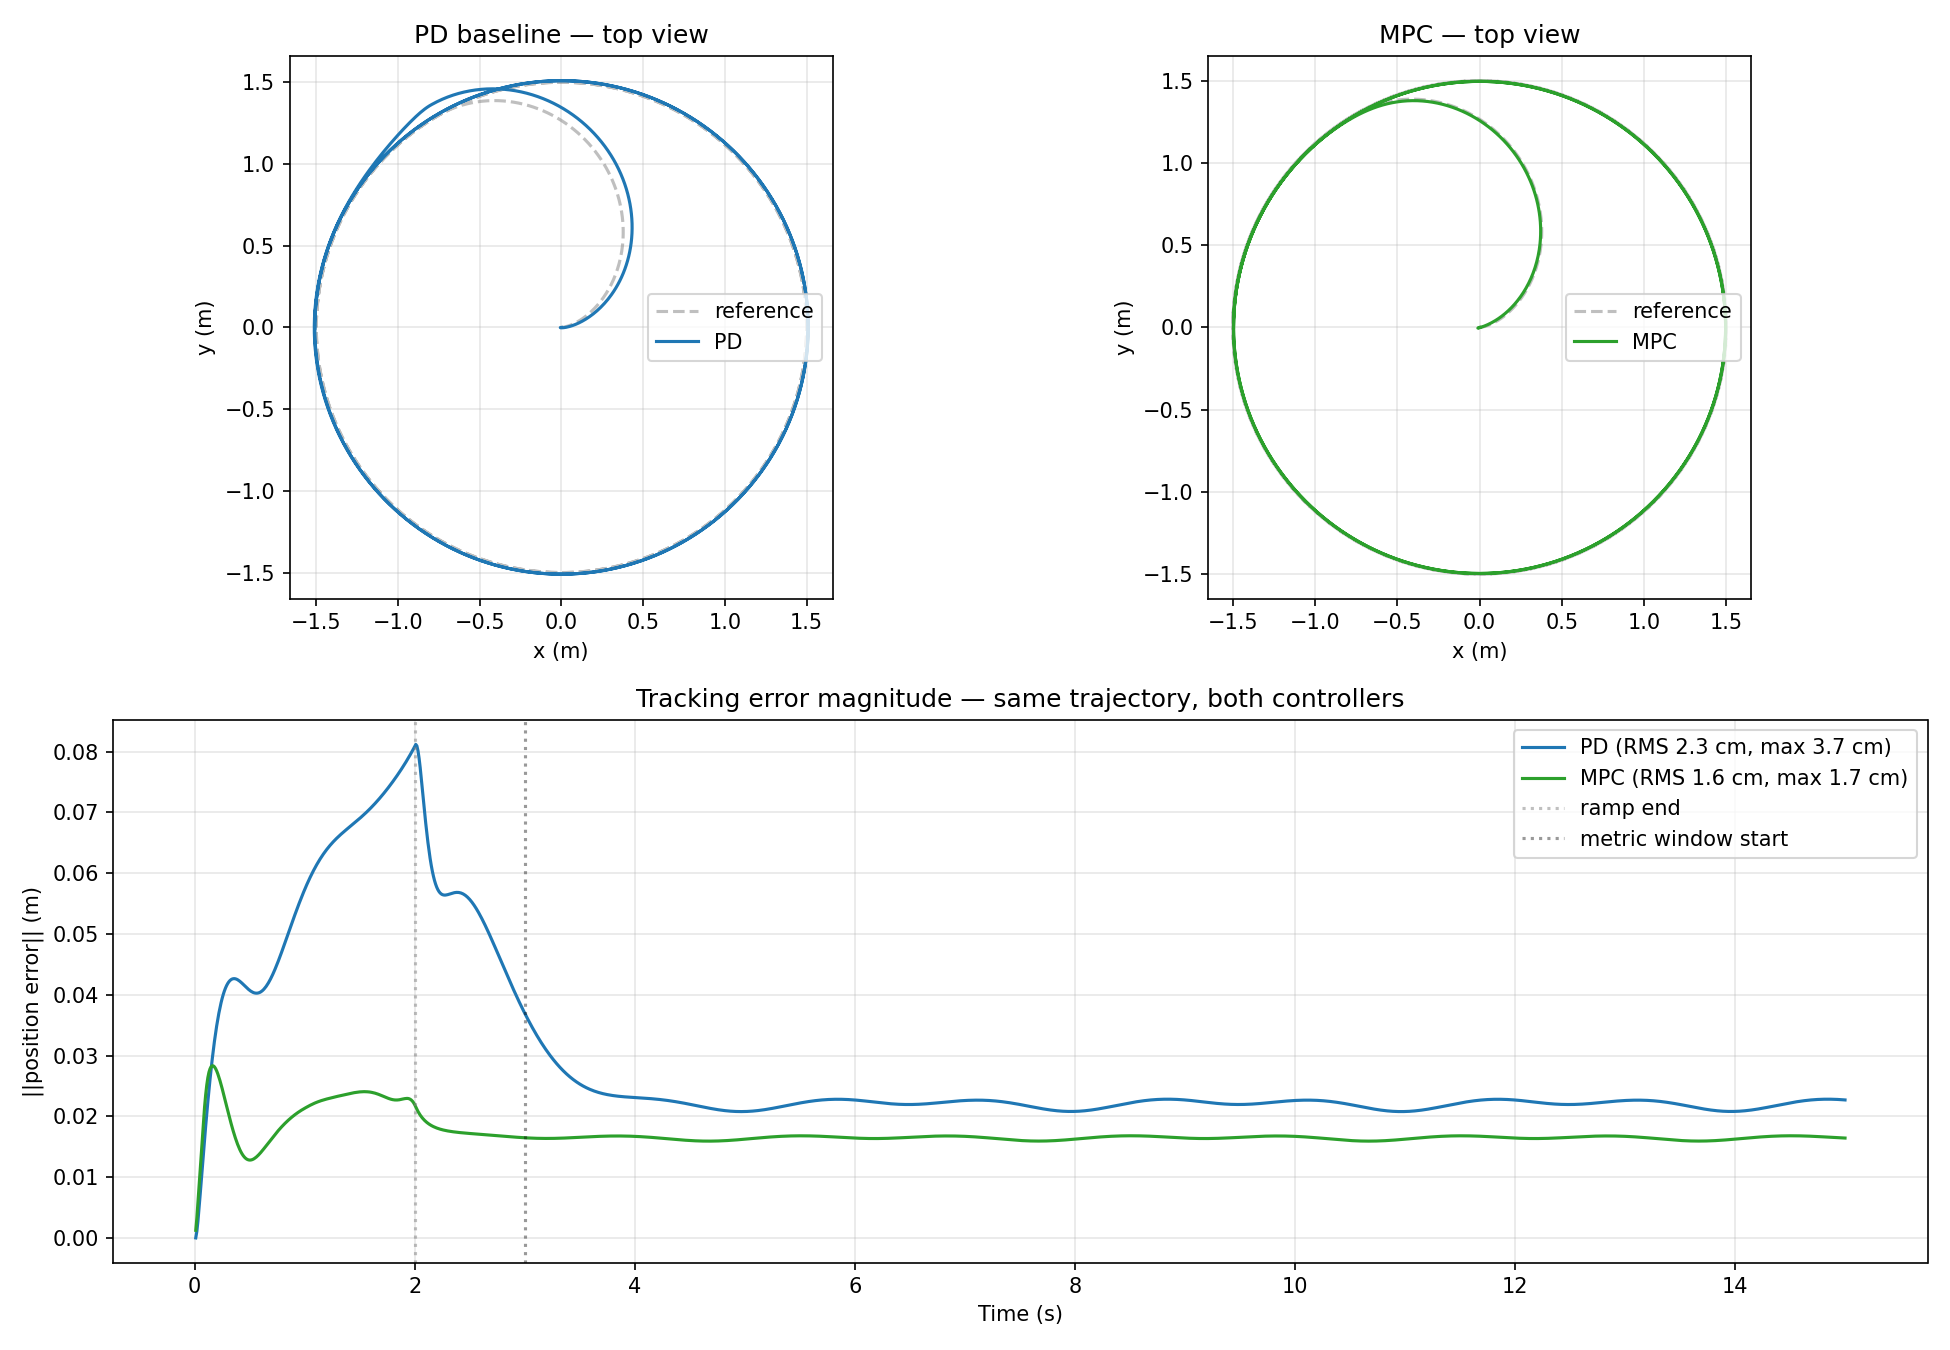
\includegraphics[width=0.95\columnwidth]{figures/comparison_pd_vs_mpc.png}
\caption{Tracking comparison between the cascaded PD baseline (red) and the nominal MPC (blue) on the 1.5 m radius, 1.57 m/s circle trajectory. The MPC reduces both RMS and maximum tracking error relative to PD on identical simulator conditions. The reference is shown as a dashed gray curve.}
\label{fig:pdvsmpc}
\end{figure}

The 1.65 cm RMS error of the nominal MPC on the unperturbed plant is the reference floor against which all perturbation experiments in Section V and recovery experiments in Section VIII are measured. The gap between this floor and the perturbed-plant tracking error defines what a learned residual can in principle recover.



\section{Perturbation Characterization}

\subsection{Perturbation Types and Implementation}
This section characterizes how the nominal MPC degrades under five distinct model-mismatch types, each isolated to a single physical mechanism. The MPC, the inner loop, the motor mixer, and the reference trajectory are unchanged across all experiments. Only MuJoCo's plant is perturbed. Mass and inertia perturbations are applied once at model load by scaling the corresponding body parameter. Drag is applied at every physics step as an external force $\mathbf{F}_{\text{drag}} = -b\, \mathbf{v}$ through MuJoCo's \texttt{xfrc\_applied} interface, where $b$ is the linear drag coefficient and $\mathbf{v}$ is the world-frame velocity. Motor lag is implemented as a first-order filter on each commanded motor thrust with time constant $\tau$, so that the actual thrust $T_{\text{actual}}$ evolves as
\begin{equation}
T_{\text{actual}}^{(k+1)} = T_{\text{actual}}^{(k)} + \frac{\Delta t_{\text{sim}}}{\tau} \left( T_{\text{commanded}}^{(k)} - T_{\text{actual}}^{(k)} \right).
\end{equation}
Time delay is implemented as a pure transport delay on the motor command vector, buffering commands for a fixed number of simulation steps before applying them to MuJoCo. The buffer is pre-filled with the per-rotor hover thrust to avoid spurious behavior during the first $\tau_d$ seconds of each trial.

\subsection{Experimental Protocol}
Each perturbation type is swept across a range that begins at the nominal value and extends until either the controller produces qualitatively unacceptable tracking error or the trial crashes. A trial is flagged as crashed when the drone falls below 0.1 m altitude, exceeds 50 m from the origin, or exceeds 30 m/s in speed at any point during the 15-second simulation. The same circle reference described in Section III is used for all trials. Tracking error is computed over the post-ramp window between 3 s and 15 s. For motor lag and time delay, an initial coarse sweep is followed by a fine-grained sweep around the cliff region, so that the transition from stable to crashed regime is resolved at single-millisecond increments.

\subsection{Aggregate Results}
The aggregated tracking-error curves are shown in Figure~\ref{fig:perturb}. The five perturbation types produce qualitatively different degradation patterns, which is the central observation of this stage. Mass and drag degrade smoothly across their full stable range. Motor lag has a wide flat region followed by a sharp transition before crashing. Time delay has effectively zero degradation region followed by an instantaneous cliff. Inertia is nearly inert across the entire tested range, with meaningful effects appearing only at the extremes. Table~\ref{tab:perturb} summarizes the boundaries and worst-stable tracking error for each perturbation type.

\begin{figure}[t]
\centering

\includegraphics[width=0.95\columnwidth]{figures/aggregate_perturbations.png}
\caption{Tracking RMS error for the nominal MPC under each of the five perturbation types, swept independently. Each subplot shows tracking error on the y-axis and perturbation magnitude on the x-axis. The horizontal dashed line marks the unperturbed baseline of 1.65 cm. Red marks indicate trials that crashed before completing the 15-second window.}
\label{fig:perturb}
\end{figure}

\begin{table}[t]
\centering
\caption{Boundaries and degradation behavior of the five perturbation types under the nominal MPC.}
\label{tab:perturb}
\begin{tabular}{lll}
\toprule
Type & Stable range & Worst stable RMS \\
\midrule
Mass & 0.7 to 1.4 of nominal & 9.95 cm at factor 1.4 \\
Inertia & 0.5 to 2.0 of nominal & 4.13 cm at factor 0.5 \\
Drag & 0 to 2.0 N\,s/m & 13.10 cm at $b = 2.0$ \\
Motor lag & 0 to 50 ms & 12.30 cm at $\tau = 50$ ms \\
Time delay & 0 to 14 ms & 1.65 cm (flat) \\
\bottomrule
\end{tabular}
\end{table}

\subsection{Mass Perturbation}
Mass mismatch produces a symmetric V-shaped degradation pattern. Tracking error grows from the 1.65 cm baseline at the nominal mass factor of 1.0 to 9.95 cm at a mass factor of 1.4 and to 7.77 cm at a mass factor of 0.7. The asymmetry is mild: heavier drones degrade slightly more than lighter ones at the equivalent fractional perturbation. The mechanism is direct. The MPC's prediction model uses the nominal mass to convert commanded thrust into expected acceleration. When the actual mass is higher, the commanded thrust produces less acceleration than predicted, the drone sags, and the controller falls behind. When the actual mass is lower, the opposite occurs. Both directions break tracking, and neither produces instability within the tested range. No mass-perturbation trial crashed.

\subsection{Inertia Perturbation}
The inertia sweep is nearly flat across the tested range of 0.5 to 2.0 of nominal, with all stable trials producing tracking error between 1.5 and 1.7 cm. The single exception is a factor of 0.5, where the very low inertia causes mild rate-loop oscillation and the RMS error rises to 4.13 cm. Beyond a factor of 2.5, trials crash because the rate-loop bandwidth becomes insufficient to track the MPC's rate commands on the more sluggish vehicle. The near-flatness of the curve is a feature, not a bug, of the kinematic-thrust MPC formulation: the outer MPC does not include inertia in its prediction model, and the inner body-rate loop tolerates a wide range of inertia values through its proportional feedback. Inertia is therefore not a perturbation type for which the learned residual is expected to be useful, and it is omitted from the evaluation in Section VIII.

\subsection{Drag Perturbation}
Drag produces a monotonically increasing degradation curve from 1.65 cm at $b = 0$ to 13.10 cm at $b = 2.0$ N\,s/m. The curve is smooth and convex, with no cliff and no crashed trials. One unexpected feature appears at very low drag: at $b = 0.1$ N\,s/m, the tracking error is 1.18 cm, which is below the unperturbed baseline of 1.65 cm. This effect is real and reproducible. A small amount of unmodeled drag provides passive damping that smooths the MPC's high-frequency rate commands, reducing the inner-loop oscillation that otherwise sets the tracking floor. Above $b \approx 0.25$ N\,s/m, drag becomes large enough that it functions as a disturbance rather than a damping source, and tracking error rises monotonically. Drag is the cleanest example of a smoothly learnable perturbation in the suite.

\subsection{Motor Lag}
The motor lag sweep was extended with a fine-grained zoom from 30 to 65 ms in 1 ms increments to resolve the cliff transition. The result is a wide flat region from 0 to 42 ms in which tracking error is indistinguishable from the unperturbed baseline, a transition zone from 43 to 49 ms in which RMS error grows from 1.65 cm to 11.08 cm, and crashes at 50 ms and beyond. The transition is therefore not a cliff in the strict sense but rather a sharp ramp with a width of approximately 6 ms. The mechanism is that the lag time constant approaches the inner body-rate loop's characteristic period; below this threshold the loop absorbs the lag, above it the loop falls behind. The narrow transition zone is the only regime in which a learned residual has any opportunity to help, since the regions on either side are either too benign or already crashed.

\subsection{Time Delay}
Time delay produces the most aggressive cliff in the suite. Tracking error remains at the unperturbed baseline of 1.65 cm for all delays from 0 to 14 ms, and every trial at 15 ms or beyond crashes. The transition has effectively zero width at the resolution of the simulator timestep. The mechanism is the classical closed-loop delay instability: the MPC plans based on a state that is several milliseconds old, the resulting commands are slightly mis-timed, and on a high-bandwidth quadrotor the resulting positive feedback grows without bound. The absence of a smooth degradation regime means that the learned residual is not expected to have any usable signal for this perturbation type, since the only trials in the stable region are those where there is no error to recover.

\subsection{Summary}
The five perturbation types together produce three distinct degradation patterns: smooth and learnable (mass, drag), formulation-independent (inertia), and cliff-dominated (motor lag, time delay). The Stage 5 evaluation in Section VIII focuses on the smooth perturbations because they offer a graceful degradation regime in which a learned residual can in principle contribute, and includes motor lag because its narrow transition zone is the place where the residual is most likely to fail interestingly. Inertia is omitted because the controller is already robust to it through its formulation, and time delay is omitted because there is no degradation regime to evaluate against.




\section{Perturbation Characterization}

\subsection{Perturbation Types and Implementation}
This section characterizes how the nominal MPC degrades under five distinct model-mismatch types, each isolated to a single physical mechanism. The MPC, the inner loop, the motor mixer, and the reference trajectory are unchanged across all experiments. Only MuJoCo's plant is perturbed. Mass and inertia perturbations are applied once at model load by scaling the corresponding body parameter. Drag is applied at every physics step as an external force $\mathbf{F}_{\text{drag}} = -b\, \mathbf{v}$ through MuJoCo's \texttt{xfrc\_applied} interface, where $b$ is the linear drag coefficient and $\mathbf{v}$ is the world-frame velocity. Motor lag is implemented as a first-order filter on each commanded motor thrust with time constant $\tau$, so that the actual thrust $T_{\text{actual}}$ evolves as
\begin{equation}
T_{\text{actual}}^{(k+1)} = T_{\text{actual}}^{(k)} + \frac{\Delta t_{\text{sim}}}{\tau} \left( T_{\text{commanded}}^{(k)} - T_{\text{actual}}^{(k)} \right).
\end{equation}
Time delay is implemented as a pure transport delay on the motor command vector, buffering commands for a fixed number of simulation steps before applying them to MuJoCo. The buffer is pre-filled with the per-rotor hover thrust to avoid spurious behavior during the first $\tau_d$ seconds of each trial.

\subsection{Experimental Protocol}
Each perturbation type is swept across a range that begins at the nominal value and extends until either the controller produces qualitatively unacceptable tracking error or the trial crashes. A trial is flagged as crashed when the drone falls below 0.1 m altitude, exceeds 50 m from the origin, or exceeds 30 m/s in speed at any point during the 15-second simulation. The same circle reference described in Section III is used for all trials. Tracking error is computed over the post-ramp window between 3 s and 15 s. For motor lag and time delay, an initial coarse sweep is followed by a fine-grained sweep around the cliff region, so that the transition from stable to crashed regime is resolved at single-millisecond increments.

\subsection{Aggregate Results}
The aggregated tracking-error curves are shown in Figure~\ref{fig:perturb}. The five perturbation types produce qualitatively different degradation patterns, which is the central observation of this stage. Mass and drag degrade smoothly across their full stable range. Motor lag has a wide flat region followed by a sharp transition before crashing. Time delay has effectively zero degradation region followed by an instantaneous cliff. Inertia is nearly inert across the entire tested range, with meaningful effects appearing only at the extremes. Table~\ref{tab:perturb} summarizes the boundaries and worst-stable tracking error for each perturbation type.

\begin{figure}[t]
\centering

\includegraphics[width=0.95\columnwidth]{figures/aggregate_perturbations.png}
\caption{Tracking RMS error for the nominal MPC under each of the five perturbation types, swept independently. Each subplot shows tracking error on the y-axis and perturbation magnitude on the x-axis. The horizontal dashed line marks the unperturbed baseline of 1.65 cm. Red marks indicate trials that crashed before completing the 15-second window.}
\label{fig:perturb}
\end{figure}

\begin{table}[t]
\centering
\caption{Boundaries and degradation behavior of the five perturbation types under the nominal MPC.}
\label{tab:perturb}
\begin{tabular}{lll}
\toprule
Type & Stable range & Worst stable RMS \\
\midrule
Mass & 0.7 to 1.4 of nominal & 9.95 cm at factor 1.4 \\
Inertia & 0.5 to 2.0 of nominal & 4.13 cm at factor 0.5 \\
Drag & 0 to 2.0 N\,s/m & 13.10 cm at $b = 2.0$ \\
Motor lag & 0 to 50 ms & 12.30 cm at $\tau = 50$ ms \\
Time delay & 0 to 14 ms & 1.65 cm (flat) \\
\bottomrule
\end{tabular}
\end{table}

\subsection{Mass Perturbation}
Mass mismatch produces a symmetric V-shaped degradation pattern. Tracking error grows from the 1.65 cm baseline at the nominal mass factor of 1.0 to 9.95 cm at a mass factor of 1.4 and to 7.77 cm at a mass factor of 0.7. The asymmetry is mild: heavier drones degrade slightly more than lighter ones at the equivalent fractional perturbation. The mechanism is direct. The MPC's prediction model uses the nominal mass to convert commanded thrust into expected acceleration. When the actual mass is higher, the commanded thrust produces less acceleration than predicted, the drone sags, and the controller falls behind. When the actual mass is lower, the opposite occurs. Both directions break tracking, and neither produces instability within the tested range. No mass-perturbation trial crashed.

\subsection{Inertia Perturbation}
The inertia sweep is nearly flat across the tested range of 0.5 to 2.0 of nominal, with all stable trials producing tracking error between 1.5 and 1.7 cm. The single exception is a factor of 0.5, where the very low inertia causes mild rate-loop oscillation and the RMS error rises to 4.13 cm. Beyond a factor of 2.5, trials crash because the rate-loop bandwidth becomes insufficient to track the MPC's rate commands on the more sluggish vehicle. The near-flatness of the curve is a feature, not a bug, of the kinematic-thrust MPC formulation: the outer MPC does not include inertia in its prediction model, and the inner body-rate loop tolerates a wide range of inertia values through its proportional feedback. Inertia is therefore not a perturbation type for which the learned residual is expected to be useful, and it is omitted from the evaluation in Section VIII.

\subsection{Drag Perturbation}
Drag produces a monotonically increasing degradation curve from 1.65 cm at $b = 0$ to 13.10 cm at $b = 2.0$ N\,s/m. The curve is smooth and convex, with no cliff and no crashed trials. One unexpected feature appears at very low drag: at $b = 0.1$ N\,s/m, the tracking error is 1.18 cm, which is below the unperturbed baseline of 1.65 cm. This effect is real and reproducible. A small amount of unmodeled drag provides passive damping that smooths the MPC's high-frequency rate commands, reducing the inner-loop oscillation that otherwise sets the tracking floor. Above $b \approx 0.25$ N\,s/m, drag becomes large enough that it functions as a disturbance rather than a damping source, and tracking error rises monotonically. Drag is the cleanest example of a smoothly learnable perturbation in the suite.

\subsection{Motor Lag}
The motor lag sweep was extended with a fine-grained zoom from 30 to 65 ms in 1 ms increments to resolve the cliff transition. The result is a wide flat region from 0 to 42 ms in which tracking error is indistinguishable from the unperturbed baseline, a transition zone from 43 to 49 ms in which RMS error grows from 1.65 cm to 11.08 cm, and crashes at 50 ms and beyond. The transition is therefore not a cliff in the strict sense but rather a sharp ramp with a width of approximately 6 ms. The mechanism is that the lag time constant approaches the inner body-rate loop's characteristic period; below this threshold the loop absorbs the lag, above it the loop falls behind. The narrow transition zone is the only regime in which a learned residual has any opportunity to help, since the regions on either side are either too benign or already crashed.

\subsection{Time Delay}
Time delay produces the most aggressive cliff in the suite. Tracking error remains at the unperturbed baseline of 1.65 cm for all delays from 0 to 14 ms, and every trial at 15 ms or beyond crashes. The transition has effectively zero width at the resolution of the simulator timestep. The mechanism is the classical closed-loop delay instability: the MPC plans based on a state that is several milliseconds old, the resulting commands are slightly mis-timed, and on a high-bandwidth quadrotor the resulting positive feedback grows without bound. The absence of a smooth degradation regime means that the learned residual is not expected to have any usable signal for this perturbation type, since the only trials in the stable region are those where there is no error to recover.

\subsection{Summary}
The five perturbation types together produce three distinct degradation patterns: smooth and learnable (mass, drag), formulation-independent (inertia), and cliff-dominated (motor lag, time delay). The Stage 5 evaluation in Section VIII focuses on the smooth perturbations because they offer a graceful degradation regime in which a learned residual can in principle contribute, and includes motor lag because its narrow transition zone is the place where the residual is most likely to fail interestingly. Inertia is omitted because the controller is already robust to it through its formulation, and time delay is omitted because there is no degradation regime to evaluate against.




\section{Feedforward Residual Control Architecture}

\subsection{In-Constraint Formulation: Attempt and Failure}
The theoretically natural way to integrate a learned residual into MPC is to embed the residual inside the optimization as part of the dynamics constraint:
\begin{equation}
\mathbf{x}_{k+1} = \mathbf{f}_{\text{nominal}}(\mathbf{x}_k, \mathbf{u}_k) + \mathbf{r}(\mathbf{x}_k, \mathbf{u}_k)
\end{equation}
where $\mathbf{r}$ is the CasADi-converted residual function from Section VI. This formulation allows the optimizer to anticipate the residual over the full prediction horizon, which is the principal theoretical advantage of in-constraint integration over feedforward alternatives. We implemented this formulation, verified that the residual CasADi function is correctly inserted into the constraint graph, and ran it against the same circle reference used in all previous experiments under a mass-factor-1.2 perturbation.

The result was that IPOPT exceeded its maximum iteration limit on every solve in the production closed-loop simulation. The failure persisted across multiple mitigation passes: switching activations from ReLU to $\tanh$, clamping the input normalization standard deviation, loosening the primary tolerance from $10^{-3}$ to $10^{-2}$, loosening the acceptable tolerance from $10^{-1}$ to $10$, raising the maximum iteration cap from 100 to 300, switching to a monotone $\mu$ strategy with $\mu_{\text{init}} = 10^{-4}$, switching to limited-memory Hessian approximation, and introducing a residual scaling factor in the range 0.0 to 1.0. None of these mitigations produced a stable closed loop.

A standalone diagnostic was constructed to isolate the failure mode from the closed-loop dynamics. The diagnostic builds a single residual-augmented MPC problem at the reference initial condition and asks IPOPT to solve it from scratch, with reference-seeded initial guess and a generous maximum-iteration budget. The diagnostic results are reported in Table~\ref{tab:diagnostic}. The solver converges at every residual scale, with iteration count growing from 3 at scale 0.0 (nominal MPC) to 61 at scale 1.0 (full residual). The standalone diagnostic therefore confirms that the residual-augmented problem is feasible and that the optimizer can solve it with sufficient budget.

\begin{table}[t]
\centering
\caption{Standalone diagnostic of the in-constraint residual MPC at varying residual scale. The solver converges at every scale but iteration count grows substantially with residual influence.}
\label{tab:diagnostic}
\begin{tabular}{ccc}
\toprule
Residual scale & IPOPT iterations & Solve time (s) \\
\midrule
0.0 (nominal) & 3 & 0.32 \\
0.01 & 3 & 3.68 \\
0.1 & 9 & 3.55 \\
0.5 & 56 & 4.32 \\
1.0 & 61 & 4.33 \\
\bottomrule
\end{tabular}
\end{table}

The gap between the diagnostic and the production closed loop is the warm-start. In the production setting, each MPC solve is initialized from the shifted previous solution. When the previous solve has not fully converged within its budget, the warm-start lies in a region of the optimization landscape from which the next solve cannot recover. The shifted warm-start interacts with the residual's contribution to the constraint Jacobian in a way that destabilizes the interior-point iteration sequence: the local quadratic approximation that IPOPT constructs at each iteration is dominated by the residual's nonlinearity rather than by the nominal dynamics, and the trust-region steps shrink without producing descent. Over a series of consecutive solves, the controller produces partial solutions of degrading quality until it returns hover commands as a fallback, at which point the closed loop is effectively open and the drone drifts. The root cause is therefore not the residual model, the CasADi conversion, the solver tolerances, or any of the mitigations we tried individually, but rather the interaction between the residual's Jacobian structure and the warm-started interior-point iteration in a closed loop with a short MPC update period.

We document this failure mode because it has important implications for any practical deployment of in-constraint residual MPC on resource-constrained platforms using general-purpose interior-point solvers, and because the literature is largely silent on the specific failure pattern we observed. Implementations of in-constraint residual MPC in prior work \cite{torrente2021data, salzmann2023real} have used custom real-time iteration schemes, dedicated solvers, or GPU acceleration that were not available in our setting. The failure is therefore conditional on the deployment context rather than fundamental to the formulation.

\subsection{Feedforward Architecture}
The feedforward residual control architecture used for the evaluation in Section VIII is shown in Figure~\ref{fig:arch}. The MPC of Section IV runs unchanged with the nominal dynamics in its constraints and produces a four-dimensional control command. After each MPC solve, the residual model is queried at the current state and the MPC's first control. The predicted vertical velocity component of the residual is converted into a thrust correction, which is added to the MPC's commanded thrust before the four-motor mixer. The MPC itself is unaware of the residual; the residual is applied externally as a feedforward signal. The body-rate inner loop and the motor mixer of Section IV operate without modification.

\begin{figure}[t]
\centering
\begin{tikzpicture}[
  node distance=4mm and 6mm,
  block/.style={draw, rounded corners=2pt, minimum width=20mm, minimum height=7mm, align=center, font=\small},
  data/.style={draw, dashed, rounded corners=2pt, minimum width=20mm, minimum height=7mm, align=center, font=\small\itshape},
  small/.style={font=\footnotesize},
  arr/.style={-Stealth, thick}
]
\node[data] (rollout) {Rollouts under\\ 21 perturbations};
\node[block, below=of rollout] (train) {Train residual MLP\\ ($\tanh$, 5641 params)};
\node[block, below=of train] (casadi) {Convert to CasADi\\ symbolic function};
\node[block, right=18mm of casadi] (residual) {Residual model\\ $\mathbf{r}(\mathbf{x},\mathbf{u})$};
\node[block, right=8mm of residual] (mpc) {Nominal MPC\\ (Sec.~IV)};
\node[block, above=of mpc] (ref) {Reference\\ trajectory};
\node[block, below=of mpc] (correct) {Thrust correction\\ $\Delta T = -m\, r_{v_z}/\Delta t_{\text{sim}}$};
\node[block, below=of correct] (mixer) {Body-rate loop\\ + motor mixer};
\node[block, below=of mixer] (plant) {MuJoCo plant\\ (perturbed)};

\draw[arr] (rollout) -- (train);
\draw[arr] (train) -- (casadi);
\draw[arr] (casadi) -- (residual);
\draw[arr] (ref) -- (mpc);
\draw[arr] (mpc) -- node[right, small] {$\mathbf{u}_{\text{mpc}}$} (correct);
\draw[arr] (residual.north) |- ($(mpc.east)+(0,-2mm)$);
\draw[arr] (residual) -- (correct.east);
\draw[arr] (correct) -- node[right, small] {$\mathbf{u}_{\text{corr}}$} (mixer);
\draw[arr] (mixer) -- (plant);
\draw[arr] (plant.west) -- ++(-15mm,0) |- node[left, small, near start] {$\mathbf{x}$} (mpc.west);
\draw[arr] (plant.west) -- ++(-15mm,0) |- (residual.west);
\end{tikzpicture}
\caption{System architecture. The offline pipeline on the left collects rollouts, trains the residual MLP, and converts it to a CasADi symbolic function. The online pipeline on the right runs the nominal MPC unchanged, queries the residual at the current state and MPC control, and applies a feedforward thrust correction before the body-rate loop and motor mixer.}
\label{fig:arch}
\end{figure}

\subsection{Thrust Correction Derivation}
The residual $\mathbf{r}(\mathbf{x}, \mathbf{u})$ predicts the one-step deviation of the perturbed plant from the nominal model. The sixth component of the residual, $r_{v_z}$, is the predicted vertical velocity deviation over one simulator timestep. If the MPC's commanded thrust were the only actuation channel modifying vertical velocity, the predicted velocity deviation could be canceled by applying an additional thrust $\Delta T$ such that
\begin{equation}
\frac{\Delta T}{m}\, \Delta t_{\text{sim}} = -r_{v_z}
\end{equation}
which rearranges to
\begin{equation}
\Delta T = -\frac{m\, r_{v_z}}{\Delta t_{\text{sim}}}.
\end{equation}
The corrected thrust passed to the motor mixer is
\begin{equation}
T_{\text{applied}} = \mathrm{clip}\!\left(T_{\text{mpc}} + \Delta T,\; 0,\; T_{\max}\right)
\end{equation}
where the clip enforces the physical actuator bounds. The thrust correction is further bounded to $|\Delta T| \leq 5$ N as a safety limit to prevent unphysical commands during transients or out-of-distribution residual predictions. The 5 N bound corresponds to approximately one third of the nominal hover thrust of 13 N and is sufficiently large that it does not activate during normal closed-loop operation under any of the perturbations within the training distribution.

\subsection{Properties of the Architecture}
The feedforward architecture has three properties that bear on the evaluation. First, the MPC is solved with its original constraints, so the solver behavior is identical to the nominal MPC of Section IV. Mean solve time stays at 4.2 ms across all perturbation regimes, and no closed-loop failures of the type described in Section VII-A occur. Second, the residual correction acts on a single channel (vertical thrust) of the four-dimensional control vector. Perturbations whose dominant effect is on horizontal velocity or on angular dynamics are therefore expected to receive less correction than perturbations whose effect appears in vertical velocity. This single-channel design is a deliberate scope choice: it isolates the simplest possible correction architecture and exposes how its performance varies with the structural match between perturbation type and correction channel. Third, the architecture is fully decoupled. The MPC, the residual model, and the correction logic each can be replaced or modified independently without affecting the others. The trained residual model is the same model used in the failed in-constraint attempt; only the integration changes.



\section{Evaluation}

\subsection{Protocol}
The feedforward residual architecture is evaluated against the perturbation suite from Section V. The mass, drag, and motor lag types are swept; inertia is omitted because the controller is structurally robust to it, and time delay is omitted because there is no smooth degradation regime in which any correction architecture can contribute. For each perturbation level within each type, three trials are run on the 15-second circle reference: the nominal MPC on the unperturbed plant (the reference floor), the nominal MPC on the perturbed plant (the degraded baseline), and the feedforward residual controller on the perturbed plant (the recovery candidate). The reference floor is run once per perturbation type at the beginning of the sweep. Tracking root mean square error is computed over the post-ramp window between 3 s and 15 s. The gap closure for each perturbation level is defined as
\begin{equation}
\text{gap closure} = \frac{\text{RMS}_{\text{nominal,perturbed}} - \text{RMS}_{\text{residual,perturbed}}}{\text{RMS}_{\text{nominal,perturbed}} - \text{RMS}_{\text{floor}}} \times 100\%.
\end{equation}
A gap closure of 100 percent corresponds to full recovery of the tracking error to the unperturbed floor. A negative value indicates the residual has increased the tracking error.

\subsection{Mass Perturbation}
The mass sweep covers eight factors from 0.7 to 1.4 of nominal. The results are listed in Table~\ref{tab:mass}. The feedforward residual recovers between 80 and 92 percent of the tracking error gap across the entire tested range. Recovery is highest at moderate perturbations (mass factor 0.9 and 1.1, both at 92 percent) and slightly lower at the extremes (0.7 and 1.4, at 84 and 80 percent respectively). The asymmetry is consistent with the training distribution: rollouts at extreme mass factors had higher trajectory variation and produced slightly noisier residual targets, but the model nonetheless generalizes across the full range.

\begin{table}[t]
\centering
\caption{Tracking error and gap closure for the mass perturbation sweep.}
\label{tab:mass}
\begin{tabular}{cccc}
\toprule
Mass factor & Nominal RMS (cm) & Residual RMS (cm) & Gap closure \\
\midrule
0.7 & 7.77 & 2.64 & 84\% \\
0.8 & 5.37 & 2.10 & 88\% \\
0.9 & 3.09 & 1.77 & 92\% \\
1.0 & 1.65 & 1.64 & --- \\
1.1 & 2.87 & 1.75 & 92\% \\
1.2 & 5.11 & 2.07 & 88\% \\
1.3 & 7.51 & 2.60 & 84\% \\
1.4 & 9.95 & 3.34 & 80\% \\
\bottomrule
\end{tabular}
\end{table}

The thrust correction applied by the residual scales nearly linearly with the mass perturbation, ranging from $-2.90$ N at mass factor 0.7 to $+3.66$ N at mass factor 1.4. The slope is approximately 0.95 N per 0.1 mass factor, consistent with the physical intuition that heavier drones require additional thrust and lighter drones require less. At the nominal mass factor of 1.0 the mean correction is $-0.04$ N, which confirms that the residual model does not introduce a systematic bias when the dynamics match the nominal model. The residual contribution at this point is essentially zero, and the feedforward controller's RMS of 1.64 cm matches the floor of 1.65 cm to within measurement noise.

\subsection{Drag Perturbation}
The drag sweep covers seven coefficients from 0.0 to 2.0 N\,s/m. The results are listed in Table~\ref{tab:drag}. The feedforward residual produces gap closure within $\pm 2$ percent across the entire range, which is statistically indistinguishable from zero. The thrust correction across all drag levels stays under 0.05 N in magnitude, confirming that the residual's vertical-velocity prediction under drag is negligible.

\begin{table}[t]
\centering
\caption{Tracking error and gap closure for the drag perturbation sweep.}
\label{tab:drag}
\begin{tabular}{cccc}
\toprule
Drag $b$ (N\,s/m) & Nominal RMS (cm) & Residual RMS (cm) & Gap closure \\
\midrule
0.0 & 1.65 & 1.64 & --- \\
0.1 & 1.18 & 1.17 & $-1\%$ \\
0.3 & 1.48 & 1.48 & $-2\%$ \\
0.5 & 2.74 & 2.73 & 0\% \\
1.0 & 6.27 & 6.26 & 0\% \\
1.5 & 9.75 & 9.75 & 0\% \\
2.0 & 13.10 & 13.11 & 0\% \\
\bottomrule
\end{tabular}
\end{table}

The reason is structural rather than a model deficiency. Linear drag $\mathbf{F}_{\text{drag}} = -b\, \mathbf{v}$ produces a force whose magnitude scales with the full velocity vector, but on the circle trajectory the vehicle's vertical velocity is held near zero by design. The drag force therefore manifests almost entirely on the horizontal axes, and the corresponding velocity residuals appear in $v_x$ and $v_y$, not in $v_z$. The residual model itself predicts these horizontal residuals with $R^2$ above 0.97 (Section VI), but the feedforward correction acts only on the vertical thrust channel, which has no mechanism to influence horizontal velocity over the timescale of a single MPC step. The result is an instructive negative outcome: the residual model is informative about the perturbation, but the correction architecture cannot route that information to where it is needed. This is the architecture's "does nothing" regime: not a failure of the learned model, but a structural mismatch between what the residual knows and what the controller can act on.

\subsection{Motor Lag}
The motor lag sweep is the most informative of the three. Stage 4 characterized motor lag as a perturbation with a wide flat region (0--42 ms) followed by a narrow transition zone (43--49 ms) and crashes at 50 ms and beyond. The Stage 5 sweep was therefore designed to span both the flat region and the transition zone in 1 ms increments, in order to resolve where and how the residual interacts with each regime. The results are listed in Table~\ref{tab:lag}.

\begin{table}[t]
\centering
\caption{Tracking error for the motor lag sweep. The flat region (0--42 ms) shows no degradation under either controller. The transition zone (43--49 ms) shows the residual destabilization effect.}
\label{tab:lag}
\begin{tabular}{cccc}
\toprule
Lag $\tau$ (ms) & Nominal RMS (cm) & Residual RMS (cm) & $\Delta$ over nominal \\
\midrule
0 & 1.65 & 1.64 & --- \\
20 & 1.65 & 1.64 & --- \\
40 & 1.65 & 1.64 & --- \\
42 & 1.65 & 1.64 & --- \\
43 & 1.65 & 1.98 & $+20\%$ \\
44 & 3.17 & 4.60 & $+45\%$ \\
45 & 5.14 & 6.65 & $+29\%$ \\
46 & 6.79 & 8.39 & $+24\%$ \\
47 & 8.26 & 10.02 & $+21\%$ \\
48 & 9.73 & 12.09 & $+24\%$ \\
49 & 11.08 & 12.76 & $+15\%$ \\
\bottomrule
\end{tabular}
\end{table}

In the flat region (0 to 42 ms) the nominal MPC tracks at the unperturbed floor and the residual controller produces no measurable change. This is the expected outcome: there is no error gap for the residual to close, and the model correctly outputs a near-zero correction.

In the transition zone (43 to 49 ms) the residual controller produces tracking error that is between 15 and 45 percent higher than the nominal degraded error at the same perturbation level. The mean thrust correction within this zone reaches $-4$ N at $\tau = 48$ ms, near the safety clip of $\pm 5$ N. The residual is therefore actively driving thrust commands in a direction that worsens tracking. This is the architecture's "hurts" regime, and the mechanism is worth examining in detail.

Under severe motor lag the commanded thrust trails the actual thrust by a delay comparable to the inner-loop time constant. The drone tends to sag below the reference altitude because the lagging motors cannot maintain hover thrust during transients. The residual sees the resulting vertical velocity discrepancy and, applying its training-time mapping from (state, control) to predicted residual, outputs a negative correction to anticipate further sag. The feedforward architecture passes this correction to the motor mixer, which reduces commanded thrust. The actual outcome is that the drone falls further, because the correct action in this regime is to command more thrust, not less, to compensate for the lagging motors. The residual model is extrapolating from a training distribution in which the closed loop was effectively stable. In the transition zone, this assumption no longer holds, and the model's mapping has the wrong sign relative to what the controller needs.

This finding has two implications. First, the destabilization is not a defect of the model fit; the model accurately reproduces the training distribution. It is a defect of the closed-loop assumption embedded in the residual definition. The residual treats the observed dynamics as ground truth, but when the closed loop itself becomes marginal, the observed dynamics are not what would result from feedforward correction. Second, the destabilization is concentrated in a narrow band (6 ms wide) immediately before the cliff to instability. Detecting this band at runtime is in principle possible if a side channel reports inner-loop bandwidth health, but no such signal is used in the present feedforward architecture. The result is that the architecture must be deployed with awareness that perturbation regimes close to closed-loop stability boundaries are unsafe for the residual to operate in.

\subsection{Aggregate View}
Figure~\ref{fig:agg} consolidates the three sweeps and the time delay reference into a single 2$\times$2 panel. The mass panel shows the symmetric V-shape of the nominal degradation collapsed to a nearly flat residual curve. The drag panel shows the nominal and residual curves essentially overlapping. The motor lag panel shows the residual curve below the nominal curve in the flat region and visibly above the nominal curve in the transition zone, with the destabilization band shaded. The time delay panel shows both curves coinciding at the floor up to the cliff at 15 ms.

\begin{figure}[t]
\centering

\includegraphics[width=0.95\columnwidth]{figures/stage5_aggregate.png}
\caption{Tracking RMS error for the nominal MPC (red) and the feedforward residual MPC (blue) across the four perturbation types, with the unperturbed baseline shown as a dashed green line. The mass panel shows the matched regime (80--92 percent gap closure). The drag panel shows the mismatched regime (no recovery). The motor lag panel shows the cliff-edge regime with the destabilization zone highlighted. The time delay panel shows the no-degradation regime below the cliff.}
\label{fig:agg}
\end{figure}

\subsection{Computational Cost}
The feedforward architecture adds approximately 27 microseconds per MPC step for the residual evaluation. The MPC solve itself is unchanged from the nominal controller, with mean solve time of 4.2 ms and maximum solve time below 75 ms across all perturbation trials. Total per-step computation including residual evaluation, MPC solve, body-rate loop, and motor mixer remains within the 10 ms budget for 100 Hz operation on the CPU-only setup.



\section{Evaluation}

\subsection{Protocol}
The feedforward residual architecture is evaluated against the perturbation suite from Section V. The mass, drag, and motor lag types are swept; inertia is omitted because the controller is structurally robust to it, and time delay is omitted because there is no smooth degradation regime in which any correction architecture can contribute. For each perturbation level within each type, three trials are run on the 15-second circle reference: the nominal MPC on the unperturbed plant (the reference floor), the nominal MPC on the perturbed plant (the degraded baseline), and the feedforward residual controller on the perturbed plant (the recovery candidate). The reference floor is run once per perturbation type at the beginning of the sweep. Tracking root mean square error is computed over the post-ramp window between 3 s and 15 s. The gap closure for each perturbation level is defined as
\begin{equation}
\text{gap closure} = \frac{\text{RMS}_{\text{nominal,perturbed}} - \text{RMS}_{\text{residual,perturbed}}}{\text{RMS}_{\text{nominal,perturbed}} - \text{RMS}_{\text{floor}}} \times 100\%.
\end{equation}
A gap closure of 100 percent corresponds to full recovery of the tracking error to the unperturbed floor. A negative value indicates the residual has increased the tracking error.

\subsection{Mass Perturbation}
The mass sweep covers eight factors from 0.7 to 1.4 of nominal. The results are listed in Table~\ref{tab:mass}. The feedforward residual recovers between 80 and 92 percent of the tracking error gap across the entire tested range. Recovery is highest at moderate perturbations (mass factor 0.9 and 1.1, both at 92 percent) and slightly lower at the extremes (0.7 and 1.4, at 84 and 80 percent respectively). The asymmetry is consistent with the training distribution: rollouts at extreme mass factors had higher trajectory variation and produced slightly noisier residual targets, but the model nonetheless generalizes across the full range.

\begin{table}[t]
\centering
\caption{Tracking error and gap closure for the mass perturbation sweep.}
\label{tab:mass}
\begin{tabular}{cccc}
\toprule
Mass factor & Nominal RMS (cm) & Residual RMS (cm) & Gap closure \\
\midrule
0.7 & 7.77 & 2.64 & 84\% \\
0.8 & 5.37 & 2.10 & 88\% \\
0.9 & 3.09 & 1.77 & 92\% \\
1.0 & 1.65 & 1.64 & --- \\
1.1 & 2.87 & 1.75 & 92\% \\
1.2 & 5.11 & 2.07 & 88\% \\
1.3 & 7.51 & 2.60 & 84\% \\
1.4 & 9.95 & 3.34 & 80\% \\
\bottomrule
\end{tabular}
\end{table}

The thrust correction applied by the residual scales nearly linearly with the mass perturbation, ranging from $-2.90$ N at mass factor 0.7 to $+3.66$ N at mass factor 1.4. The slope is approximately 0.95 N per 0.1 mass factor, consistent with the physical intuition that heavier drones require additional thrust and lighter drones require less. At the nominal mass factor of 1.0 the mean correction is $-0.04$ N, which confirms that the residual model does not introduce a systematic bias when the dynamics match the nominal model. The residual contribution at this point is essentially zero, and the feedforward controller's RMS of 1.64 cm matches the floor of 1.65 cm to within measurement noise.

\subsection{Drag Perturbation}
The drag sweep covers seven coefficients from 0.0 to 2.0 N\,s/m. The results are listed in Table~\ref{tab:drag}. The feedforward residual produces gap closure within $\pm 2$ percent across the entire range, which is statistically indistinguishable from zero. The thrust correction across all drag levels stays under 0.05 N in magnitude, confirming that the residual's vertical-velocity prediction under drag is negligible.

\begin{table}[t]
\centering
\caption{Tracking error and gap closure for the drag perturbation sweep.}
\label{tab:drag}
\begin{tabular}{cccc}
\toprule
Drag $b$ (N\,s/m) & Nominal RMS (cm) & Residual RMS (cm) & Gap closure \\
\midrule
0.0 & 1.65 & 1.64 & --- \\
0.1 & 1.18 & 1.17 & $-1\%$ \\
0.3 & 1.48 & 1.48 & $-2\%$ \\
0.5 & 2.74 & 2.73 & 0\% \\
1.0 & 6.27 & 6.26 & 0\% \\
1.5 & 9.75 & 9.75 & 0\% \\
2.0 & 13.10 & 13.11 & 0\% \\
\bottomrule
\end{tabular}
\end{table}

The reason is structural rather than a model deficiency. Linear drag $\mathbf{F}_{\text{drag}} = -b\, \mathbf{v}$ produces a force whose magnitude scales with the full velocity vector, but on the circle trajectory the vehicle's vertical velocity is held near zero by design. The drag force therefore manifests almost entirely on the horizontal axes, and the corresponding velocity residuals appear in $v_x$ and $v_y$, not in $v_z$. The residual model itself predicts these horizontal residuals with $R^2$ above 0.97 (Section VI), but the feedforward correction acts only on the vertical thrust channel, which has no mechanism to influence horizontal velocity over the timescale of a single MPC step. The result is an instructive negative outcome: the residual model is informative about the perturbation, but the correction architecture cannot route that information to where it is needed. This is the architecture's "does nothing" regime: not a failure of the learned model, but a structural mismatch between what the residual knows and what the controller can act on.

\subsection{Motor Lag}
The motor lag sweep is the most informative of the three. Stage 4 characterized motor lag as a perturbation with a wide flat region (0--42 ms) followed by a narrow transition zone (43--49 ms) and crashes at 50 ms and beyond. The Stage 5 sweep was therefore designed to span both the flat region and the transition zone in 1 ms increments, in order to resolve where and how the residual interacts with each regime. The results are listed in Table~\ref{tab:lag}.

\begin{table}[t]
\centering
\caption{Tracking error for the motor lag sweep. The flat region (0--42 ms) shows no degradation under either controller. The transition zone (43--49 ms) shows the residual destabilization effect.}
\label{tab:lag}
\begin{tabular}{cccc}
\toprule
Lag $\tau$ (ms) & Nominal RMS (cm) & Residual RMS (cm) & $\Delta$ over nominal \\
\midrule
0 & 1.65 & 1.64 & --- \\
20 & 1.65 & 1.64 & --- \\
40 & 1.65 & 1.64 & --- \\
42 & 1.65 & 1.64 & --- \\
43 & 1.65 & 1.98 & $+20\%$ \\
44 & 3.17 & 4.60 & $+45\%$ \\
45 & 5.14 & 6.65 & $+29\%$ \\
46 & 6.79 & 8.39 & $+24\%$ \\
47 & 8.26 & 10.02 & $+21\%$ \\
48 & 9.73 & 12.09 & $+24\%$ \\
49 & 11.08 & 12.76 & $+15\%$ \\
\bottomrule
\end{tabular}
\end{table}

In the flat region (0 to 42 ms) the nominal MPC tracks at the unperturbed floor and the residual controller produces no measurable change. This is the expected outcome: there is no error gap for the residual to close, and the model correctly outputs a near-zero correction.

In the transition zone (43 to 49 ms) the residual controller produces tracking error that is between 15 and 45 percent higher than the nominal degraded error at the same perturbation level. The mean thrust correction within this zone reaches $-4$ N at $\tau = 48$ ms, near the safety clip of $\pm 5$ N. The residual is therefore actively driving thrust commands in a direction that worsens tracking. This is the architecture's "hurts" regime, and the mechanism is worth examining in detail.

Under severe motor lag the commanded thrust trails the actual thrust by a delay comparable to the inner-loop time constant. The drone tends to sag below the reference altitude because the lagging motors cannot maintain hover thrust during transients. The residual sees the resulting vertical velocity discrepancy and, applying its training-time mapping from (state, control) to predicted residual, outputs a negative correction to anticipate further sag. The feedforward architecture passes this correction to the motor mixer, which reduces commanded thrust. The actual outcome is that the drone falls further, because the correct action in this regime is to command more thrust, not less, to compensate for the lagging motors. The residual model is extrapolating from a training distribution in which the closed loop was effectively stable. In the transition zone, this assumption no longer holds, and the model's mapping has the wrong sign relative to what the controller needs.

This finding has two implications. First, the destabilization is not a defect of the model fit; the model accurately reproduces the training distribution. It is a defect of the closed-loop assumption embedded in the residual definition. The residual treats the observed dynamics as ground truth, but when the closed loop itself becomes marginal, the observed dynamics are not what would result from feedforward correction. Second, the destabilization is concentrated in a narrow band (6 ms wide) immediately before the cliff to instability. Detecting this band at runtime is in principle possible if a side channel reports inner-loop bandwidth health, but no such signal is used in the present feedforward architecture. The result is that the architecture must be deployed with awareness that perturbation regimes close to closed-loop stability boundaries are unsafe for the residual to operate in.

\subsection{Aggregate View}
Figure~\ref{fig:agg} consolidates the three sweeps and the time delay reference into a single 2$\times$2 panel. The mass panel shows the symmetric V-shape of the nominal degradation collapsed to a nearly flat residual curve. The drag panel shows the nominal and residual curves essentially overlapping. The motor lag panel shows the residual curve below the nominal curve in the flat region and visibly above the nominal curve in the transition zone, with the destabilization band shaded. The time delay panel shows both curves coinciding at the floor up to the cliff at 15 ms.

\begin{figure}[t]
\centering

\includegraphics[width=0.95\columnwidth]{figures/stage5_aggregate.png}
\caption{Tracking RMS error for the nominal MPC (red) and the feedforward residual MPC (blue) across the four perturbation types, with the unperturbed baseline shown as a dashed green line. The mass panel shows the matched regime (80--92 percent gap closure). The drag panel shows the mismatched regime (no recovery). The motor lag panel shows the cliff-edge regime with the destabilization zone highlighted. The time delay panel shows the no-degradation regime below the cliff.}
\label{fig:agg}
\end{figure}

\subsection{Computational Cost}
The feedforward architecture adds approximately 27 microseconds per MPC step for the residual evaluation. The MPC solve itself is unchanged from the nominal controller, with mean solve time of 4.2 ms and maximum solve time below 75 ms across all perturbation trials. Total per-step computation including residual evaluation, MPC solve, body-rate loop, and motor mixer remains within the 10 ms budget for 100 Hz operation on the CPU-only setup.

\bibliographystyle{IEEEtran}
\bibliography{references}


@article{faessler2018differential,
  author    = {Matthias Faessler and Antonio Franchi and Davide Scaramuzza},
  title     = {Differential Flatness of Quadrotor Dynamics Subject to Rotor Drag for Accurate Tracking of High-Speed Trajectories},
  journal   = {IEEE Robotics and Automation Letters},
  volume    = {3},
  number    = {2},
  pages     = {620--626},
  year      = {2018},
  doi       = {10.1109/LRA.2017.2776353}
}

@article{torrente2021data,
  author    = {Guillem Torrente and Elia Kaufmann and Philipp Foehn and Davide Scaramuzza},
  title     = {Data-Driven MPC for Quadrotors},
  journal   = {IEEE Robotics and Automation Letters},
  volume    = {6},
  number    = {2},
  pages     = {3769--3776},
  year      = {2021},
  doi       = {10.1109/LRA.2021.3061307}
}

@article{salzmann2023real,
  author    = {Tim Salzmann and Elia Kaufmann and Jon Arrizabalaga and Marco Pavone and Davide Scaramuzza and Markus Ryll},
  title     = {Real-Time Neural {MPC}: Deep Learning Model Predictive Control for Quadrotors and Agile Robotic Platforms},
  journal   = {IEEE Robotics and Automation Letters},
  volume    = {8},
  number    = {4},
  pages     = {2397--2404},
  year      = {2023},
  doi       = {10.1109/LRA.2023.3246839}
}

@article{saviolo2023learning,
  author    = {Alessandro Saviolo and Giuseppe Loianno},
  title     = {Learning Quadrotor Dynamics for Precise, Safe, and Agile Flight Control},
  journal   = {Annual Reviews in Control},
  volume    = {55},
  pages     = {45--60},
  year      = {2023},
  doi       = {10.1016/j.arcontrol.2023.03.009}
}

@article{saviolo2022physics,
  author    = {Alessandro Saviolo and Guanrui Li and Giuseppe Loianno},
  title     = {Physics-Inspired Temporal Learning of Quadrotor Dynamics for Accurate Model Predictive Trajectory Tracking},
  journal   = {IEEE Robotics and Automation Letters},
  volume    = {7},
  number    = {4},
  pages     = {10256--10263},
  year      = {2022},
  doi       = {10.1109/LRA.2022.3192609}
}

@article{hewing2020learning,
  author    = {Lukas Hewing and Kim P. Wabersich and Marcel Menner and Melanie N. Zeilinger},
  title     = {Learning-Based Model Predictive Control: Toward Safe Learning in Control},
  journal   = {Annual Review of Control, Robotics, and Autonomous Systems},
  volume    = {3},
  pages     = {269--296},
  year      = {2020},
  doi       = {10.1146/annurev-control-090419-075625}
}

@article{hewing2018cautious,
  author    = {Lukas Hewing and Juraj Kabzan and Melanie N. Zeilinger},
  title     = {Cautious Model Predictive Control Using {Gaussian} Process Regression},
  journal   = {IEEE Transactions on Control Systems Technology},
  volume    = {28},
  number    = {6},
  pages     = {2736--2743},
  year      = {2020},
  doi       = {10.1109/TCST.2019.2949757}
}

@inproceedings{shi2019neural,
  author    = {Guanya Shi and Xichen Shi and Michael O'Connell and Rose Yu and Kamyar Azizzadenesheli and Anima Anandkumar and Yisong Yue and Soon-Jo Chung},
  title     = {Neural Lander: Stable Drone Landing Control Using Learned Dynamics},
  booktitle = {Proc. IEEE International Conference on Robotics and Automation (ICRA)},
  pages     = {9784--9790},
  year      = {2019},
  doi       = {10.1109/ICRA.2019.8794351}
}

@inproceedings{bauersfeld2021neurobem,
  author    = {Leonard Bauersfeld and Elia Kaufmann and Philipp Foehn and Sihao Sun and Davide Scaramuzza},
  title     = {{NeuroBEM}: Hybrid Aerodynamic Quadrotor Model},
  booktitle = {Proc. Robotics: Science and Systems (RSS)},
  year      = {2021},
  doi       = {10.15607/RSS.2021.XVII.042}
}

@inproceedings{punjani2015deep,
  author    = {Ali Punjani and Pieter Abbeel},
  title     = {Deep Learning Helicopter Dynamics Models},
  booktitle = {Proc. IEEE International Conference on Robotics and Automation (ICRA)},
  pages     = {3223--3230},
  year      = {2015},
  doi       = {10.1109/ICRA.2015.7139643}
}

@incollection{kamel2017linear,
  author    = {Mina Kamel and Thomas Stastny and Kostas Alexis and Roland Siegwart},
  title     = {Model Predictive Control for Trajectory Tracking of Unmanned Aerial Vehicles Using Robot Operating System},
  booktitle = {Robot Operating System ({ROS}): The Complete Reference, Vol. 2},
  editor    = {Anis Koubaa},
  publisher = {Springer International Publishing},
  pages     = {3--39},
  year      = {2017},
  doi       = {10.1007/978-3-319-54927-9_1}
}

@article{sun2022comparative,
  author    = {Sihao Sun and Angel Romero and Philipp Foehn and Elia Kaufmann and Davide Scaramuzza},
  title     = {A Comparative Study of Nonlinear {MPC} and Differential-Flatness-Based Control for Quadrotor Agile Flight},
  journal   = {IEEE Transactions on Robotics},
  volume    = {38},
  number    = {6},
  pages     = {3357--3373},
  year      = {2022},
  doi       = {10.1109/TRO.2022.3177279}
}

@article{wachter2006implementation,
  author    = {Andreas W{\"a}chter and Lorenz T. Biegler},
  title     = {On the Implementation of an Interior-Point Filter Line-Search Algorithm for Large-Scale Nonlinear Programming},
  journal   = {Mathematical Programming},
  volume    = {106},
  number    = {1},
  pages     = {25--57},
  year      = {2006},
  doi       = {10.1007/s10107-004-0559-y}
}

@article{andersson2019casadi,
  author    = {Joel A. E. Andersson and Joris Gillis and Greg Horn and James B. Rawlings and Moritz Diehl},
  title     = {{CasADi}: A Software Framework for Nonlinear Optimization and Optimal Control},
  journal   = {Mathematical Programming Computation},
  volume    = {11},
  number    = {1},
  pages     = {1--36},
  year      = {2019},
  doi       = {10.1007/s12532-018-0139-4}
}

@inproceedings{todorov2012mujoco,
  author    = {Emanuel Todorov and Tom Erez and Yuval Tassa},
  title     = {{MuJoCo}: A Physics Engine for Model-Based Control},
  booktitle = {Proc. IEEE/RSJ International Conference on Intelligent Robots and Systems (IROS)},
  pages     = {5026--5033},
  year      = {2012},
  doi       = {10.1109/IROS.2012.6386109}
}

@misc{deepmind2023menagerie,
  author    = {{Google DeepMind}},
  title     = {{MuJoCo} Menagerie: Skydio {X2}},
  year      = {2023},
  howpublished = {\url{https://github.com/google-deepmind/mujoco_menagerie/tree/main/skydio_x2}},
  note      = {Accessed: 2026}
}





\appendices

\section{Compilation of Mathematical Formulations}
This appendix consolidates the mathematical content of the paper in the order it is referenced and provides the reasoning that motivates each step. The aim is to allow a reader to trace the full derivation from continuous-time quadrotor dynamics to the closed-loop thrust correction without having to navigate between sections.

\subsection{Continuous-Time Quadrotor Dynamics}
The nominal model used by the MPC's prediction step is the standard rigid-body quadrotor with thrust as the only control over translational acceleration:
\begin{align}
\dot{\mathbf{p}} &= \mathbf{v} \tag{A.1} \\
\dot{\mathbf{v}} &= \frac{T}{m}\, \mathbf{R}(\phi, \theta, \psi)\, \mathbf{e}_3 - g\, \mathbf{e}_3 \tag{A.2} \\
\dot{\boldsymbol{\eta}} &= \mathbf{W}(\phi, \theta)\, \boldsymbol{\omega} \tag{A.3}
\end{align}
where $\mathbf{p} \in \mathbb{R}^3$ is position, $\mathbf{v} \in \mathbb{R}^3$ is linear velocity in the world frame, $\boldsymbol{\eta} = [\phi, \theta, \psi]^\top$ are Euler angles, $\boldsymbol{\omega} \in \mathbb{R}^3$ are body rates, $T$ is total thrust, $m$ is mass, $g$ is gravity, $\mathbf{R}(\phi, \theta, \psi)$ is the body-to-world rotation matrix in Z-Y-X convention, $\mathbf{W}(\phi, \theta)$ is the Euler-rate transformation matrix, and $\mathbf{e}_3 = [0, 0, 1]^\top$. This formulation deliberately omits drag, motor lag, and the inner attitude dynamics. The first two are the perturbations characterized in Section V. The third is handled by the inner body-rate loop running at the same rate as the MPC, and the MPC treats body rates as direct control inputs.

\subsection{Discrete-Time Prediction Model}
The MPC's optimization runs in discrete time. The continuous dynamics are integrated using fourth-order Runge-Kutta with prediction timestep $\Delta t = 0.05$ s:
\begin{equation}
\mathbf{x}_{k+1} = \mathbf{f}_{\text{RK4}}(\mathbf{x}_k, \mathbf{u}_k, \Delta t) \tag{A.4}
\end{equation}
RK4 is chosen over Euler because the higher integration order reduces the integration error contribution to the prediction-vs-plant gap, isolating that gap to genuine model mismatch rather than to numerical artifacts. The simulator timestep $\Delta t_{\text{sim}} = 0.01$ s is five times finer than the prediction timestep, so the simulator's own integration error is bounded well below the prediction's.

\subsection{MPC Cost Function}
The finite-horizon cost minimized at each control step is
\begin{equation}
J = \sum_{k=0}^{N-1} \left[ \mathbf{e}_k^\top \mathbf{Q}\, \mathbf{e}_k + \Delta \mathbf{u}_k^\top \mathbf{R}\, \Delta \mathbf{u}_k \right] + \mathbf{e}_N^\top \mathbf{Q}_f\, \mathbf{e}_N \tag{A.5}
\end{equation}
with $\mathbf{e}_k = \mathbf{x}_k - \mathbf{x}_{\text{ref},k}$, $\Delta \mathbf{u}_k = \mathbf{u}_k - \mathbf{u}_{\text{hover}}$, and $\mathbf{Q}_f = 10\,\mathbf{Q}$. The terminal weight $\mathbf{Q}_f$ is set ten times the running weight because a horizon of $N = 20$ at $\Delta t = 0.05$ s gives only a 1-second lookahead, and a heavier terminal weight discourages the optimizer from accepting accumulated tracking error at the end of the horizon. Centering the control deviation at $\mathbf{u}_{\text{hover}} = [m g, 0, 0, 0]^\top$ rather than at zero biases the optimizer toward the equilibrium control input, which improves both numerical conditioning and physical interpretability of the optimization.

\subsection{Motor Mixer}
The body-rate inner loop produces body-frame torques $\boldsymbol{\tau} = [\tau_x, \tau_y, \tau_z]^\top$. The motor mixer converts $(T, \boldsymbol{\tau})$ into the four-rotor thrust vector through a constant matrix derived from the cross-configuration geometry:
\begin{equation}
\mathbf{T}_{\text{motors}} = \frac{T}{4}\mathbf{1} + \mathbf{M} \begin{bmatrix} \tau_x/(4\ell_y) \\ \tau_y/(4\ell_x) \\ \tau_z/(4\kappa) \end{bmatrix} \tag{A.6}
\end{equation}
where $\mathbf{M} \in \mathbb{R}^{4 \times 3}$ encodes the rotor positions and spin directions, $\ell_x, \ell_y$ are arm lengths, and $\kappa$ is the rotor torque coefficient. The mixer is identical for the nominal MPC and the residual-augmented variant. The mixer's role is purely geometric, mapping the controller's abstract commands to physical actuator inputs.

\subsection{Residual Definition}
The residual on which the learned model is trained is the one-step deviation between the plant's evolution under the simulator and the nominal model's prediction over the same step:
\begin{equation}
\mathbf{r}(\mathbf{x}, \mathbf{u}) = \mathbf{x}^{\text{plant}}_{\text{next}} - \mathbf{f}_{\text{nominal}}(\mathbf{x}, \mathbf{u}) \tag{A.7}
\end{equation}
evaluated at the simulator timestep $\Delta t_{\text{sim}}$. This formulation aligns the residual with the data naturally collected during closed-loop rollouts and avoids requiring a separate integration scheme for training data generation.

\subsection{Input Normalization with Clamp}
Each input dimension $i$ of the MLP is normalized as
\begin{equation}
\tilde{x}_i = \frac{x_i - \mu_i}{\max(\sigma_i,\; \sigma_{\min})} \tag{A.8}
\end{equation}
where $\mu_i, \sigma_i$ are training-set mean and standard deviation and $\sigma_{\min} = 0.1$. The clamp is essential. The closed-loop nature of the training rollouts produces narrow training distributions on several state dimensions: $\sigma_{\psi} = 0.008$ rad and $\sigma_{v_z} = 0.053$ m/s. Without clamping, the per-dimension normalization scales unit input perturbations by factors $1/\sigma_i$ that exceed 100 on these dimensions. When the network is then inserted into an interior-point optimization, the resulting constraint-Jacobian condition number exceeds $10^6$, which causes the solver to fail with numerical instability. The clamp at 0.1 caps the amplification factor at 10 and produces a condition number near $6 \times 10^3$, which lies within the regime where standard solvers operate reliably. The 0.1 value is sufficient to span the physically meaningful range of all state dimensions while remaining large enough to ensure good conditioning.

\subsection{Thrust Correction Derivation}
The feedforward correction is derived from the residual's vertical velocity component $r_{v_z}$. The intent is to cancel the predicted one-step vertical velocity deviation by applying an additional thrust $\Delta T$ over the upcoming simulator step. Starting from the nominal vertical dynamics
\begin{equation}
\dot{v}_z = \frac{T \cos\phi \cos\theta}{m} - g \approx \frac{T}{m} - g \quad \text{(near hover)} \tag{A.9}
\end{equation}
and discretizing over a single simulator step $\Delta t_{\text{sim}}$, the additional vertical velocity produced by a thrust correction $\Delta T$ is
\begin{equation}
\Delta v_z = \frac{\Delta T}{m}\, \Delta t_{\text{sim}}. \tag{A.10}
\end{equation}
Setting this equal to $-r_{v_z}$ to cancel the predicted residual and solving for $\Delta T$:
\begin{equation}
\Delta T = -\frac{m\, r_{v_z}}{\Delta t_{\text{sim}}}. \tag{A.11}
\end{equation}
The applied thrust is the MPC's commanded thrust plus the correction, clipped to the physical actuator bound and to a safety bound of $\pm 5$ N to prevent unphysical commands during transients:
\begin{equation}
T_{\text{applied}} = \mathrm{clip}\!\left(T_{\text{mpc}} + \mathrm{clip}(\Delta T, -5, 5),\; 0,\; T_{\max}\right). \tag{A.12}
\end{equation}
The near-hover approximation in (A.9) is justified because the circle trajectory keeps the body tilt below $0.1$ rad throughout, so $\cos\phi \cos\theta$ remains within $0.5\%$ of unity. The single-channel scope (vertical only) is a deliberate restriction that exposes the architecture's regime structure: perturbations whose dominant residual signature is on $r_{v_z}$ receive a well-targeted correction, while those whose signature appears on $r_{v_x}$ or $r_{v_y}$ receive no correction at all.

\subsection{Gap Closure Metric}
For evaluation, the recovery achieved by the feedforward residual at each perturbation level is reported as the gap-closure percentage:
\begin{equation}
\text{gap closure} = \frac{\mathrm{RMS}_{\text{nom,pert}} - \mathrm{RMS}_{\text{res,pert}}}{\mathrm{RMS}_{\text{nom,pert}} - \mathrm{RMS}_{\text{floor}}} \times 100\% \tag{A.13}
\end{equation}
where $\mathrm{RMS}_{\text{floor}}$ is the unperturbed nominal-MPC tracking error of 1.65 cm, $\mathrm{RMS}_{\text{nom,pert}}$ is the nominal MPC's tracking error under the perturbation, and $\mathrm{RMS}_{\text{res,pert}}$ is the residual-augmented controller's tracking error under the same perturbation. A value of 100\% denotes full recovery to the unperturbed floor, 0\% denotes no improvement, and negative values denote that the residual has worsened performance.

\end{document}
